\documentclass[11pt]{article}
\usepackage{geometry}                
\geometry{letterpaper}                   

\usepackage{graphicx}
\usepackage{amssymb}
\usepackage{epstopdf}
\usepackage{natbib}
\usepackage{amssymb, amsmath}
\usepackage{wrapfig}
\usepackage{empheq}
\usepackage{pdfpages}



\begin{document}



\thispagestyle{empty}

\begin{center}

\includegraphics[width=5cm]{ETHlogo.eps}

\bigskip


\bigskip


\bigskip


\LARGE{ 	Lecture with Computer Exercises:\\ }
\LARGE{ Modelling and Simulating Social Systems with MATLAB\\}

\bigskip

\bigskip

\small{Project Report}\\

\bigskip

\bigskip

\bigskip

\bigskip


\begin{tabular}{|c|}
\hline
\\
\textbf{\LARGE{Cholera Epidemic in Haiti 2010}}\\
\\
\hline
\end{tabular}
\bigskip

\bigskip

\bigskip

\LARGE{Nicolas Stocker 

Benedict Borer

Benjamin Pluess 

Lukas Buehler}



\bigskip

\bigskip

\bigskip

\bigskip

\bigskip

\bigskip

\bigskip

\bigskip

Zurich\\
\today\\
\end{center}



\newpage

%%%%%%%%%%%%%%%%%%%%%%%%%%%%%%%%%%%%%%%%%%%%%%%%%

\newpage
\section*{Agreement for free-download}
\bigskip


\bigskip


\large We hereby agree to make our source code for this project freely available for download from the web pages of the SOMS chair. Furthermore, we assure that all source code is written by ourselves and is not violating any copyright restrictions.

\begin{center}

\bigskip


\bigskip


\begin{tabular}{@{}p{3.3cm}@{}p{6cm}@{}@{}p{6cm}@{}}
\begin{minipage}{3cm}

\end{minipage}
&
\begin{minipage}{6cm}
\vspace{2mm} \large Nicolas Stocker 


 \vspace{\baselineskip}

\end{minipage}
&
\begin{minipage}{6cm}

\large Benjamin Pluess

\end{minipage}
\end{tabular}

\bigskip
\bigskip
\bigskip

\begin{tabular}{@{}p{3.3cm}@{}p{6cm}@{}@{}p{6cm}@{}}
\begin{minipage}{3cm}

\end{minipage}
&
\begin{minipage}{6cm}
\vspace{2mm} \large Benedict Borer 


 \vspace{\baselineskip}

\end{minipage}
&
\begin{minipage}{6cm}

\large Lukas Buehler

\end{minipage}
\end{tabular}


\end{center}
\newpage

%%%%%%%%%%%%%%%%%%%%%%%%%%%%%%%%%%%%%%%



% IMPORTANT
% you MUST include the ETH declaration of originality here; it is available for download on the course website or at http://www.ethz.ch/faculty/exams/plagiarism/index_EN; it can be printed as pdf and should be filled out in handwriting
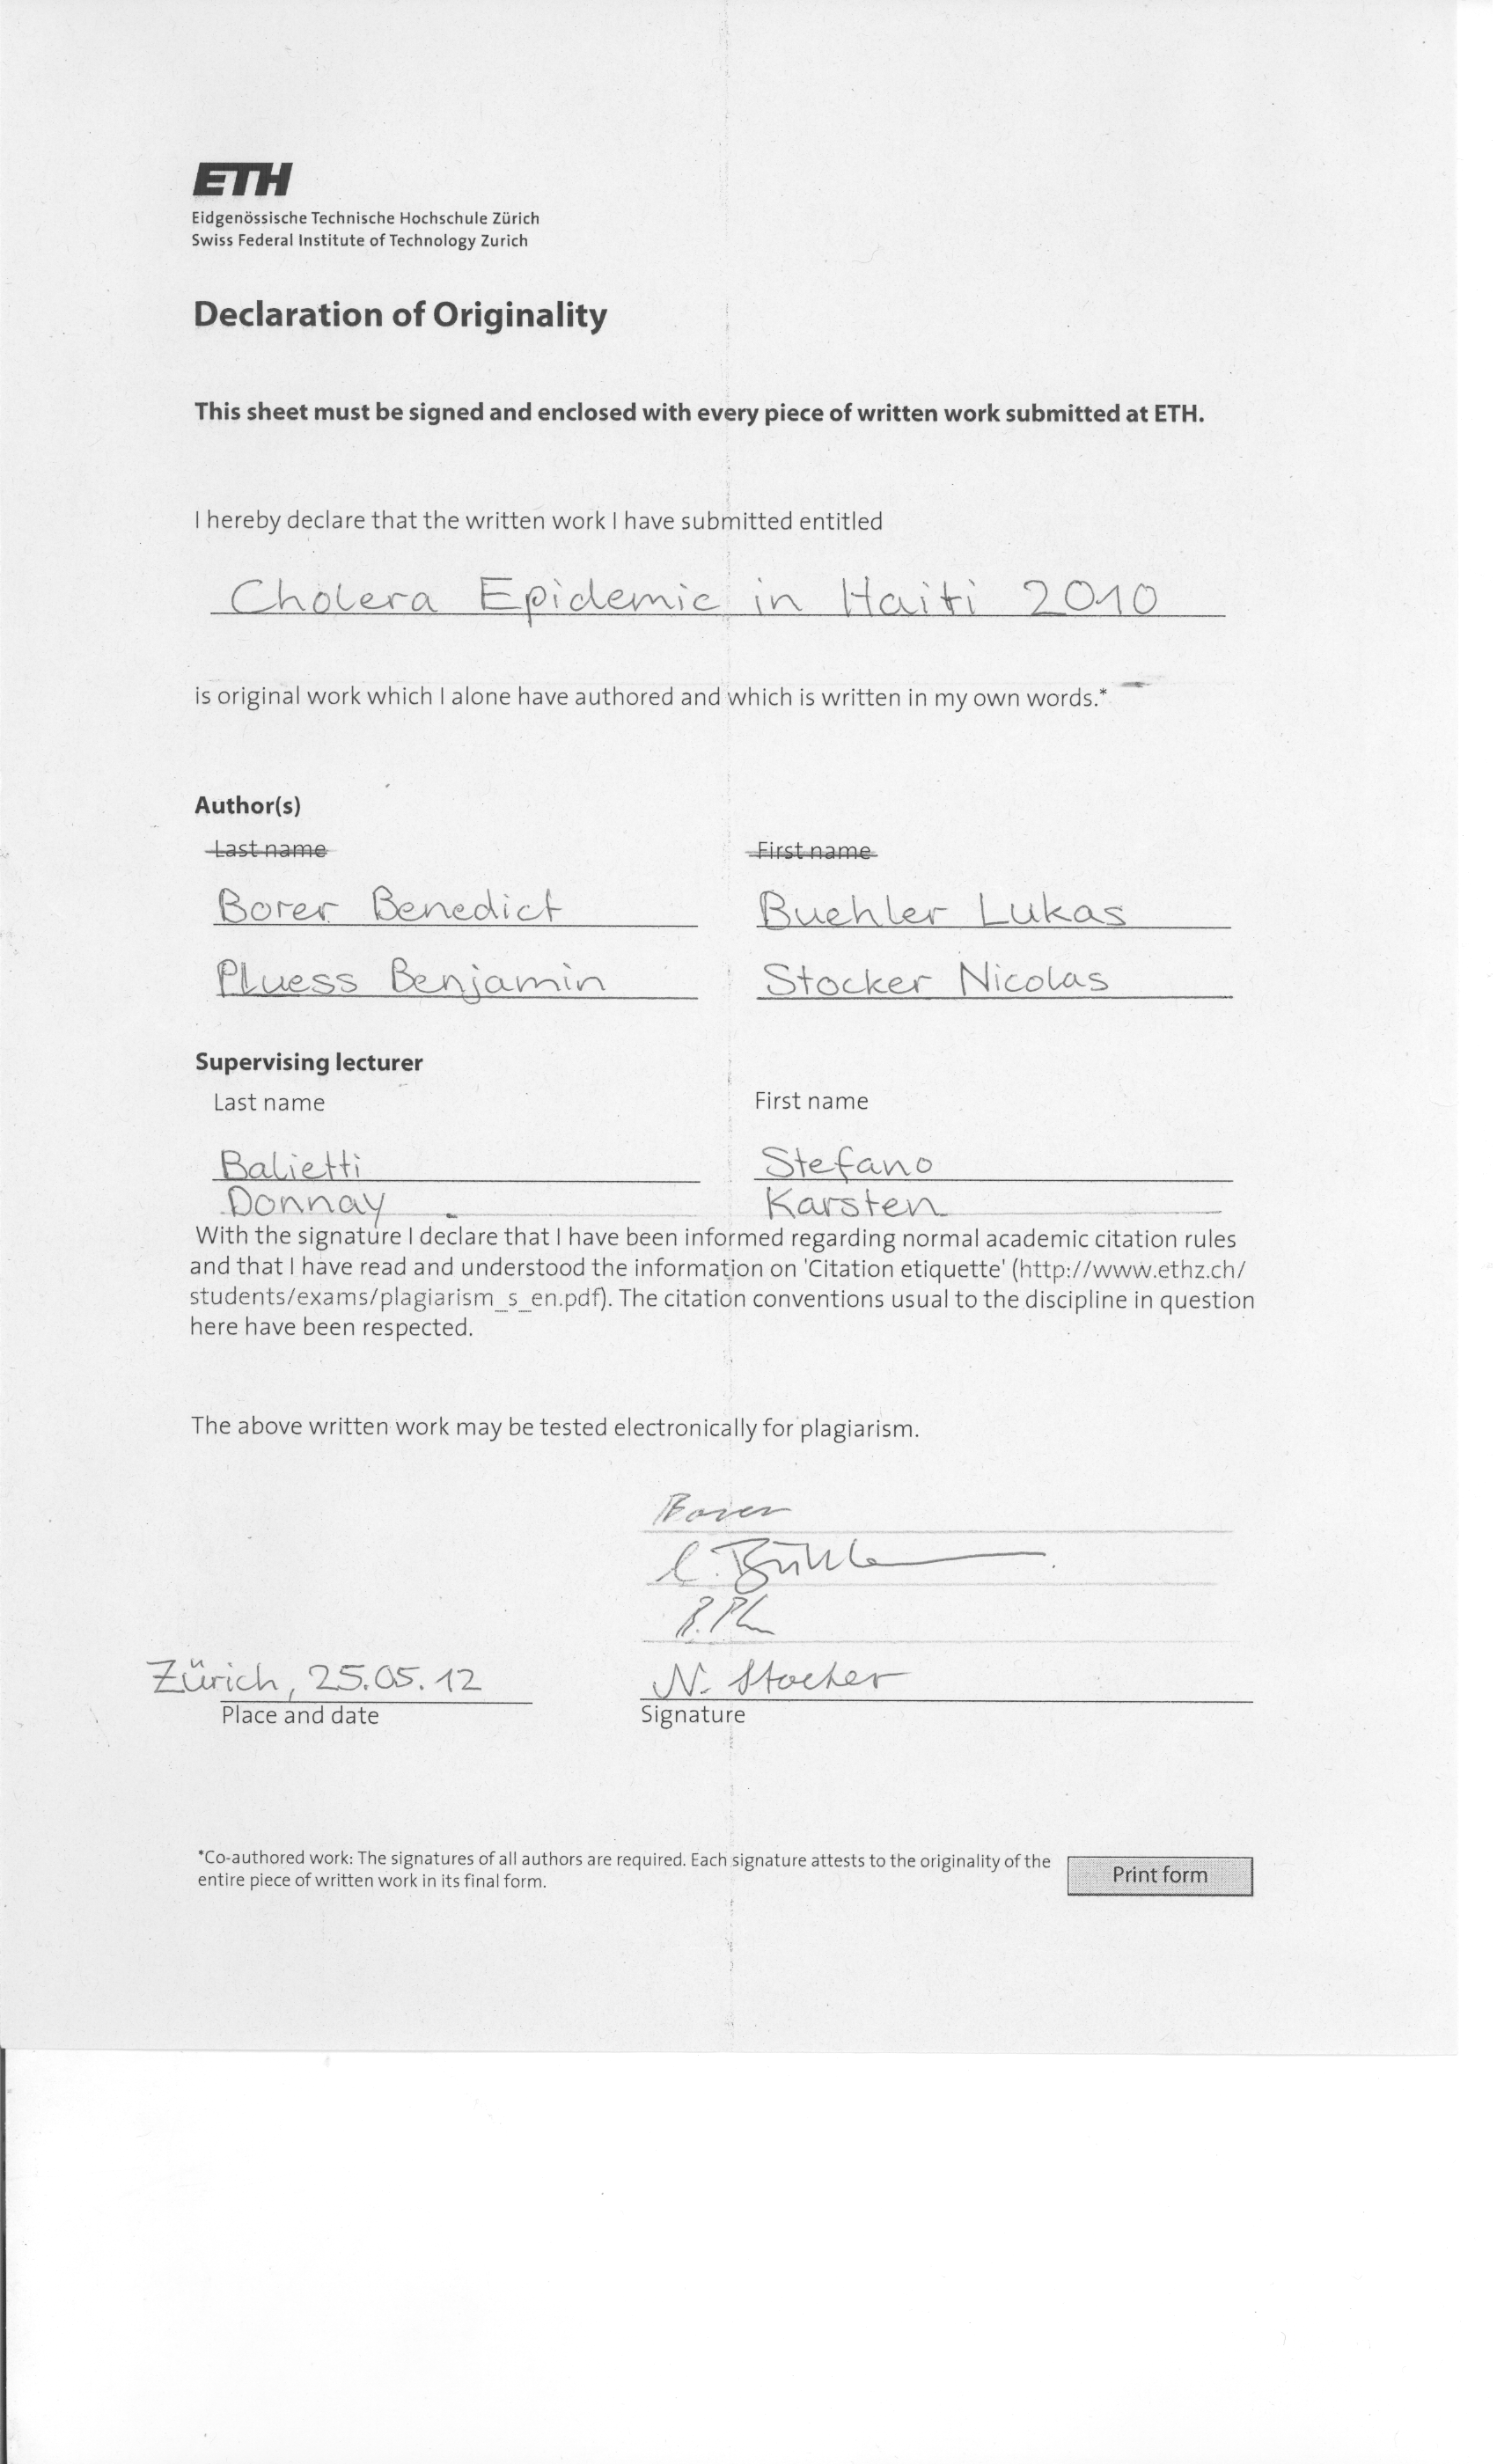
\includepdf[]{Bilder/declaration_of_originality.png}


\section*{Abstract}
Following the earthquake on 12 January 2010, a cholera epidemic broke out in the fall of the same year. Here we set out to model the propagation of the epidemic with a SIWR model as proposed by Tien et al. Due to lack of reliable data for the water quality and problems with the model equations, we build a SIR model as proposed by Kermack et al. Furthermore, to predict interdepartmental transmission, we include the same gravity weighted model as used by Tuite et al. Our model manages to predict the magnitude and spacial spread of the epidemic in many districts. The districts Grand Anse, Nord and Nord Est show an incredible increase of the removed compartment in the original data. Whilst trying to explain this increase we take a critical look at our own model, the data and the gravity weighted model. Finally we make propositions to improve the gravity weighted model as used by Tuite et al. to better model a pathogen related epidemics in the aftermath of a disaster. 



\newpage

%%%%%%%%%% Table of content %%%%%%%%%%%%%%%%%

\tableofcontents

\newpage

%%%%%%%%%%%%%%%%%%%%%%%%%%%%%%%%%%%%%%%












\newpage
\section{Individual contributions}
\begin{itemize}
\item Conception and design of model: Nicolas Stocker, Benedict Borer
\item Implementation: Benedict Borer
\item Analysis and interpretation of the data: Benedict Borer, Nicolas Stocker
\item Writing the report: Benedict Borer, Nicolas Stocker, Lukas Buehler, Benjamin Pluess
\item Revision of the report: Benedict Borer, Nicolas Stocker, Lukas Buehler, Benjamin Pluess
\item Administrative efforts: Lukas Buehler
\item Layouting: Lukas Buehler
\item Collection and assembly of data: Benjamin Pluess
\item Visualization tool: Benjamin Pluess
\end{itemize}


\newpage
\section{Introduction and Motivation}
\subsection{Introduction to Haiti, the earthquake and cholera }
\subsubsection*{The shock}


\begin{wrapfigure}{r}{0.5\textwidth}
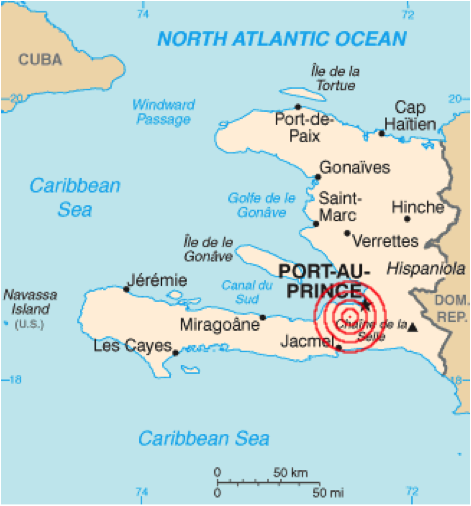
\includegraphics[width=0.48\textwidth]{Bilder/KarteHaiti.png}
\caption{Map of Haiti with the epicenter \cite{wikipedia:map}}
\label{pic:map_haiti}
\end{wrapfigure}


12 January 2010, 16.53 local time in Haiti: for an entire minute the earth shook, with a magnitude of 7.0  (on the Moment magnitude scale), with an epicenter 25 km west of Haiti's capital, Port-au-Prince. \cite{nyt:mag} Followed by at least 52 aftershocks,  this earthquake was the most dramatic in the 21st century: the Haitian government estimated that 316,000 people died \cite{web:cbc1}, one million people lost their homes, and 3.2 million were directly affected. \cite{web:ear}

\subsubsection*{Geological overview}
The earthquake was located on the active plate boundary, with the Caribbean Tectonic Plate shifting eastwards relative to the North American Plate. This caused a highly dangerous strike-slip-fault system here with the southern active Enriquillo-Plantain-Garden-fault. The earthquake was caused by a rupture of this system, which has been blocked for the past 2500 years, loading stress. \cite{web:bbc1}

\subsubsection*{Primary impacts}
As Haiti is one of the poorest countries in the western hemisphere,  the economy is highly vulnerable to natural disasters \cite{web:unicef}. In addition to earthquakes, the island of Hispaniola, shared by the Dominican Republic and Haiti, has often been struck by hurricanes. The huge devastation and damage in the whole country, but especially in the region of the capital, destroyed not only human life but also infrastructure that would have been necessary to respond to the disaster. All hospitals in the capital were destroyed, as were the air, water and land transport facilities and the communication system. Many of the public and government buildings were damaged (e.g. the National Assembly and the Palace of Justice) \cite{web:wikipedia_infra}.


\subsubsection*{The aftermath}
In the months following the earthquake, many people slept in the streets because their houses had been destroyed or they feared that their buildings would not survive further aftershocks. Slow distribution of resources resulted in violence and some people began plundering \cite{wikipedia:map}. The earthquake destroyed thousands of families, made a whole social system collapse, and destroyed economic interactions in the country. The Haitians' dramatic fight for survival began in the silent seconds after the earthquake and still goes on.


\subsubsection*{The approaching problem: cholera}
During the period of reconstruction in October 2010, Haiti was confronted by a new and dangerous problem: a cholera epidemic broke out! Cholera is a bacterial infection caused by a bacterium named \textit{“Vibro cholerae”} \citep{pacini:1959}. The symptoms are mainly watery diarrhea and vomiting, generally caused by drinking infected water. Cholera need not be lethal but requires appropriate treatment in a hospital. In Haiti, some 7025 deaths from cholera had been reported by January 2012. \cite{web:MSPP}.
The source of the disease is still not clearly identified, but localized in the Artibonite River about 100 km north of Port-Au-Prince (The affected victims had drunk water from the infected river.) Some UN investigators did research, hoping to find the real source of the epidemic, and hypothesized that the initial strain was imported by a UN peacekeeper from Nepal \cite{web:alj}. The Nepali soldiers may be the source of the outbreak as wastewater from the outhouses at their base flowed into and contaminated the Artibonite River. However, who brought the original strain to Haiti is not of primary importance, but rather to control the plague, and this is still one of the most important priorities today in Haiti.

\subsection{Motivation}
By the end of October 2010, the cholera epidemic had four out of ten Haitian departments in its grip: Artibonite, Centre, Nord and Ouest, including the capital, especially the slum district of “Cit\'{e} Soleil” \cite{web:alj2}. In the following days cholera was spread all over the country and infected thousands of people. The tragedy of Haiti is not only a “simple” earthquake rather it is the battle to rebuild a country affected by complicating circumstances such as the cholera epidemic. Our aim is to understand the fast spread of the cholera and to implement a mathematical model, which is able to predict the expansion of such an epidemic in space and time.












\newpage
\section{Description of the Model}
\subsection{SIR model by Kermack and McKendrick}
A general model for epidemics was established by Kermack and McKendrick over 80 years ago \cite{kermack:1927}. It is a representative of the so-called SIR models. SIR stands for the three groups a population is divided into: susceptible, infected and removed persons for the particular disease. The model makes the assumptions that the population size is constant, no incubation period exists - which means that individuals fall ill the moment they are infected, and that the time of infectivity is the same as the duration of the clinical disease \cite{kermack:1927}. This implies that infected individuals are always infectious and vice versa. Infected and infectious have therefore to be seen as descriptions of the same state. Because in reality these expressions are not equivalent, either one of them is used in a linguistic appropriate manner. Furthermore, after having been infected once, individuals become completely immune to the disease in question \cite{kermack:1927}. Kermack and McKendrick and have used the plague as an example of an epidemic which can be modeled by their work. Since then other epidemics have been modeled by similar frameworks that can be counted as part of the SIR models. The Kermack-McKendrick model equations are the following:

\begin{center}
\begin{minipage}[t]{0.6\textwidth}

\begin{empheq}[]{flalign}
&\dfrac{dS}{dt}=-\beta X(t)S(t)&          						 \label{eq:kermack_susceptible} \\
&\dfrac{dX}{dt}=\beta X(t)S(t)-\gamma X(t)&			             \label{eq:kermack_infectious} \\
&\dfrac{dR}{dt}=\gamma X(t)&                                      \label{eq:kermack_removed}
\end{empheq}

\end{minipage}
\end{center}
\newline


S, X and R are the numbers of susceptible, infectious and removed persons, respectively. Removed means that those people have either died from the disease or they have recovered and as a result are perfectly immune now. Either way, they are no longer candidates to become infected and they do not belong to the infectious population anymore. Here $\beta$ stands for the infection rate and $\gamma$ for the immunity (or death) rate. It is the inverse value of the average duration of infectiousness. If $\beta$ and $\gamma$ are constants, the spreading of an epidemic that is modelled with this concept can only decrease or be stopped when enough individuals have been moved from the susceptible to the removed compartment (becoming infectious and then being removed because of death or recovery); a decrease in the value of the susceptible compartment ($ S $) is going to lower the term $\beta X(t)S(t)$ which leads to a decrease of the value of infectious ($ X $), eventually stopping the epidemic.\\

\subsection{SIWR model by Tien and Earn}
For diseases that are transmitted through water and person-to-person contact, an extension of the SIR model was developed by Tien and Earn and called SIWR \cite{tien:2010}. The main difference is the introduction of a fourth compartment $ W $ which represents the waterbody. The water compartment can be contaminated by infectious people and susceptible individuals can be infected by the contaminated water compartment. This water compartment can improve the quality of predictions for diseases that are mainly transmitted through ingestion of contaminated water. Another new feature of the model is the introduction of natural death terms in every compartment with humans (all compartments expect $ W $) and a corresponding birth term in the susceptible compartment. These terms are chosen so that the total number of individuals in all compartments with humans stays constant.
The model equations are the following:

\begin{center}
\begin{minipage}[t]{0.6\textwidth}

\begin{empheq}[]{flalign}
&\dfrac{dS}{dt}=\mu N-b_{W}WS-b_{I}SX-\mu S&    			  \label{eq:SIWR_susceptible} \\
&\dfrac{dX}{dt}=b_{W}WS+b_{I}SX-\gamma I-\mu X&			  \label{eq:SIWR_infectious} \\
&\dfrac{dR}{dt}=\gamma X-\mu R&          				  \label{eq:SIWR_removed} \\                                           
&\dfrac{dW}{dt}=\alpha X-\xi W&	  						  \label{eq:SIWR_water}  
\end{empheq}
\end{minipage}
\end{center}
\newline



$ \mu $ is the parameter for natural deaths and the birth rate. Natural deaths occur in every human compartment, while all babies are born into the susceptible compartment. $ b_{W} $ represents the rate of infection by water-to-person contact whereas $ b_{I} $ is the rate of infection for person-to-person contact. $\frac{1}{\gamma } $ is the mean infectious period. So $ \gamma $ stands for the rate of infectious persons to either die or recover and become immune. In both cases those individuals change from the $ X $ to the $ R $ compartment. $ \alpha $ is the pathogen shedding rate from infectious persons into the water compartment while $ \xi $ denotes the decay rate of the particular pathogen in water.


\begin{center}
\begin{figure}
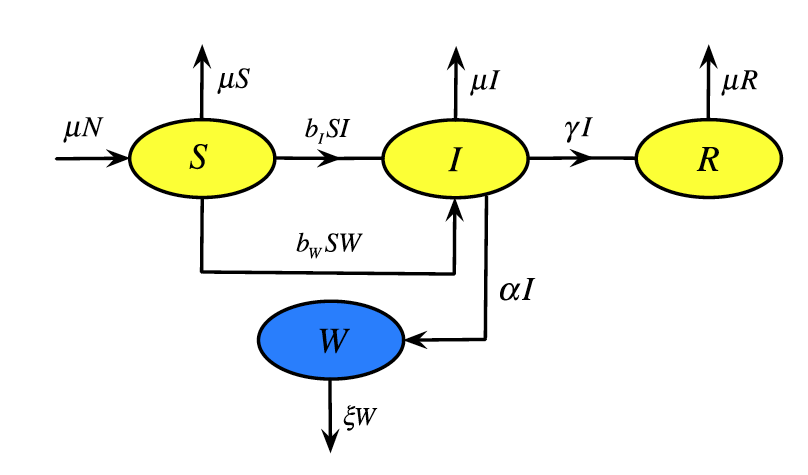
\includegraphics[width=0.8\textwidth]{Bilder/flow_diagram_SIWR.png}
\caption{SIWR model represented as a flow diagram. In addition to the SIR model there is a water compartment ($ W $) which becomes contaminated by infectious people and influencing the amount of new infections. Taken from Tien and Earn \cite{tien:2010}.}
\label{pic:flow_diagram}
\end{figure}
\end{center}

Figure \ref{pic:flow_diagram} gives an overview of the parameters and the roles they play in this model. Tien and Earn also recommend rescaling the model equations. Rescaling has some advantages, one of which being the possibility to directly compare different epidemics with different populations. Used for rescaling is the total population number $ N $. The new properties have the following relationship with the old ones: \\
\newline

\begin{center}
$ s=\dfrac{S}{N} $,	$ x=\dfrac{X}{N} $,	$ r=\dfrac{R}{N} $,	$ w=\dfrac{W}{N}\dfrac{\xi}{\alpha} $
\end{center}
\newline

\begin{center}
\begin{minipage}[t]{0.6\textwidth}
\begin{empheq}[]{flalign}
&\dfrac{ds}{dt}=\mu -\beta_{W}ws-\beta_{I}sx-\mu s&        \label{eq:SIWRrescaled_susceptible} \\
&\dfrac{dx}{dt}=\beta_{W}ws+\beta_{I}sx-\gamma x-\mu x&    \label{eq:SIWRrescaled_infectious} \\
&\dfrac{dr}{dt}=\gamma x-\mu r&                            \label{eq:SIWRrescaled_removed} \\                                           
&\dfrac{dw}{dt}=\xi (x-w)&							      \label{eq:SIWRrescaled_water}  
\end{empheq}
\end{minipage}
\end{center}
\newline



Because $ W $ was replaced by the expression $ wN\frac{\alpha}{\xi} $, which is a bit more complex than just $ wN $, parameters in expressions with a former capital $ W $ are replaced by new parameters. The differential equation for the water compartment has become simpler as only one parameter $ \xi $ is needed from now on. Two new parameters are introduced to replace $ b_{W} $ and $ b_{I} $ by $ \beta_{W}=b_{W}N\frac{\alpha}{\xi} $ and $ \beta_{I}=b_{I}N $ respectively.

\begin{quotation}
The basic reproductive number $ R_{0} $ is defined as the expected number of secondary infections that result from introducing a single infected individual into an otherwise susceptible population. $ R_{0} $ is a fundamental quantity in mathematical epidemiology, which - in the deterministic limit - dictates whether a newly invading pathogen will cause a disease outbreak  (direct quote Tien and Earn, 2010 \cite{tien:2010}).
\end{quotation}

For the SIWR model, the equation $ R_{0}=\frac{\beta_{I}+\beta_{W}}{\gamma+\mu} $ holds.
\subsection{Spatially divided SIWR model}
The SIWR model can be applied to the case of a population  that is spatially separated into different parts, which was done by Tuite \textit{et al.} for the ten districts of Haiti \cite{tuite:2011}. The only additional term which was added for this approach gives the person-to-person infections by infectious individuals of different districts. So the susceptible population of every district could be infected by the infectious population or contaminated water of their own district or infectious individuals of other districts. The last term accounts for people who move or travel around. To consider the distances between different districts a gravity-model was used \cite{tuite:2011}. Parameter $ \theta $ depends on the population of the two districts in question and on the distance between their capital cities. The concept is essentially the same as for the gravity equation: $ \Theta_{ij}=\kappa\frac{p_{i}p_{j}}{d^{n}} $. $ p_{i} $ and $ p_{j} $ are population sizes of different districts, $ d $ is given by the distance between the capital cities of the two districts in question, $ n $ influences how strong transmission depends on distance and $ \kappa $ determines how important the transmission between districts is thought to be. With this equation a between district transmission rate $ \theta_{ij} $ can be calculated for every possible constellation. With ten districts, this results in 90 different $ \theta_{ij} $, one for every possible combination. Because of the shape of Haiti, it was divided into a northern and a southern part when determining these distances. Ouest was thought to be the link between those two parts, where all travellers had to pass through. So distances between two districts that did not belong to the same part were taken as the sum of distances between the capital city of the district in the northern part and the capital city of Ouest and the distance between the capital cities of Ouest and the district in the southern part.
The equation for the model with different districts (indicated by the index $ i $) are the following:

\begin{center}
\begin{minipage}[t]{0.6\textwidth}
\begin{empheq}[]{flalign}
&\dfrac{ds_{i}}{dt}=\mu -\lambda_{i}s_{i}-\mu s_{i}& 			\label{eq:SIWRdepartments_susceptible} \\
&\dfrac{dx_{i}}{dt}=\lambda_{i}s_{i}-\gamma x_{i}-\mu x_{i}&   \label{eq:SIWRdepartments_infectious} \\
&\dfrac{dr_{i}}{dt}=\gamma x_{i}-\mu r_{i}&                    \label{eq:SIWRdepartments_removed} \\                                           
&\dfrac{dw_{i}}{dt}=\xi (x_{i}-w_{i})&					     	\label{eq:SIWRdepartments_water}  
\end{empheq}
\end{minipage}
\end{center}
\newline



The force of infection $ \lambda $ is introduced to summarize all the effects of the pathogen, such as person-to-person and water-to-person transmission within a district and person-to-person transmission between districts. While this may give a better overview about the model it hides the non-linear terms. It is important to keep in mind that $ \lambda $ includes parameters as well as variables! 

\begin{center}
\begin{minipage}[t]{0.5\textwidth}

\begin{equation}

\lambda_{i}=\beta_{W}w_{i}+\beta_{I}x_{i}+\sum\limits_{j=1}^I  \Theta_{ij}  x_{j}

\end{equation}
\end{minipage}
\end{center}
\newline



\begin{center}
\begin{figure}
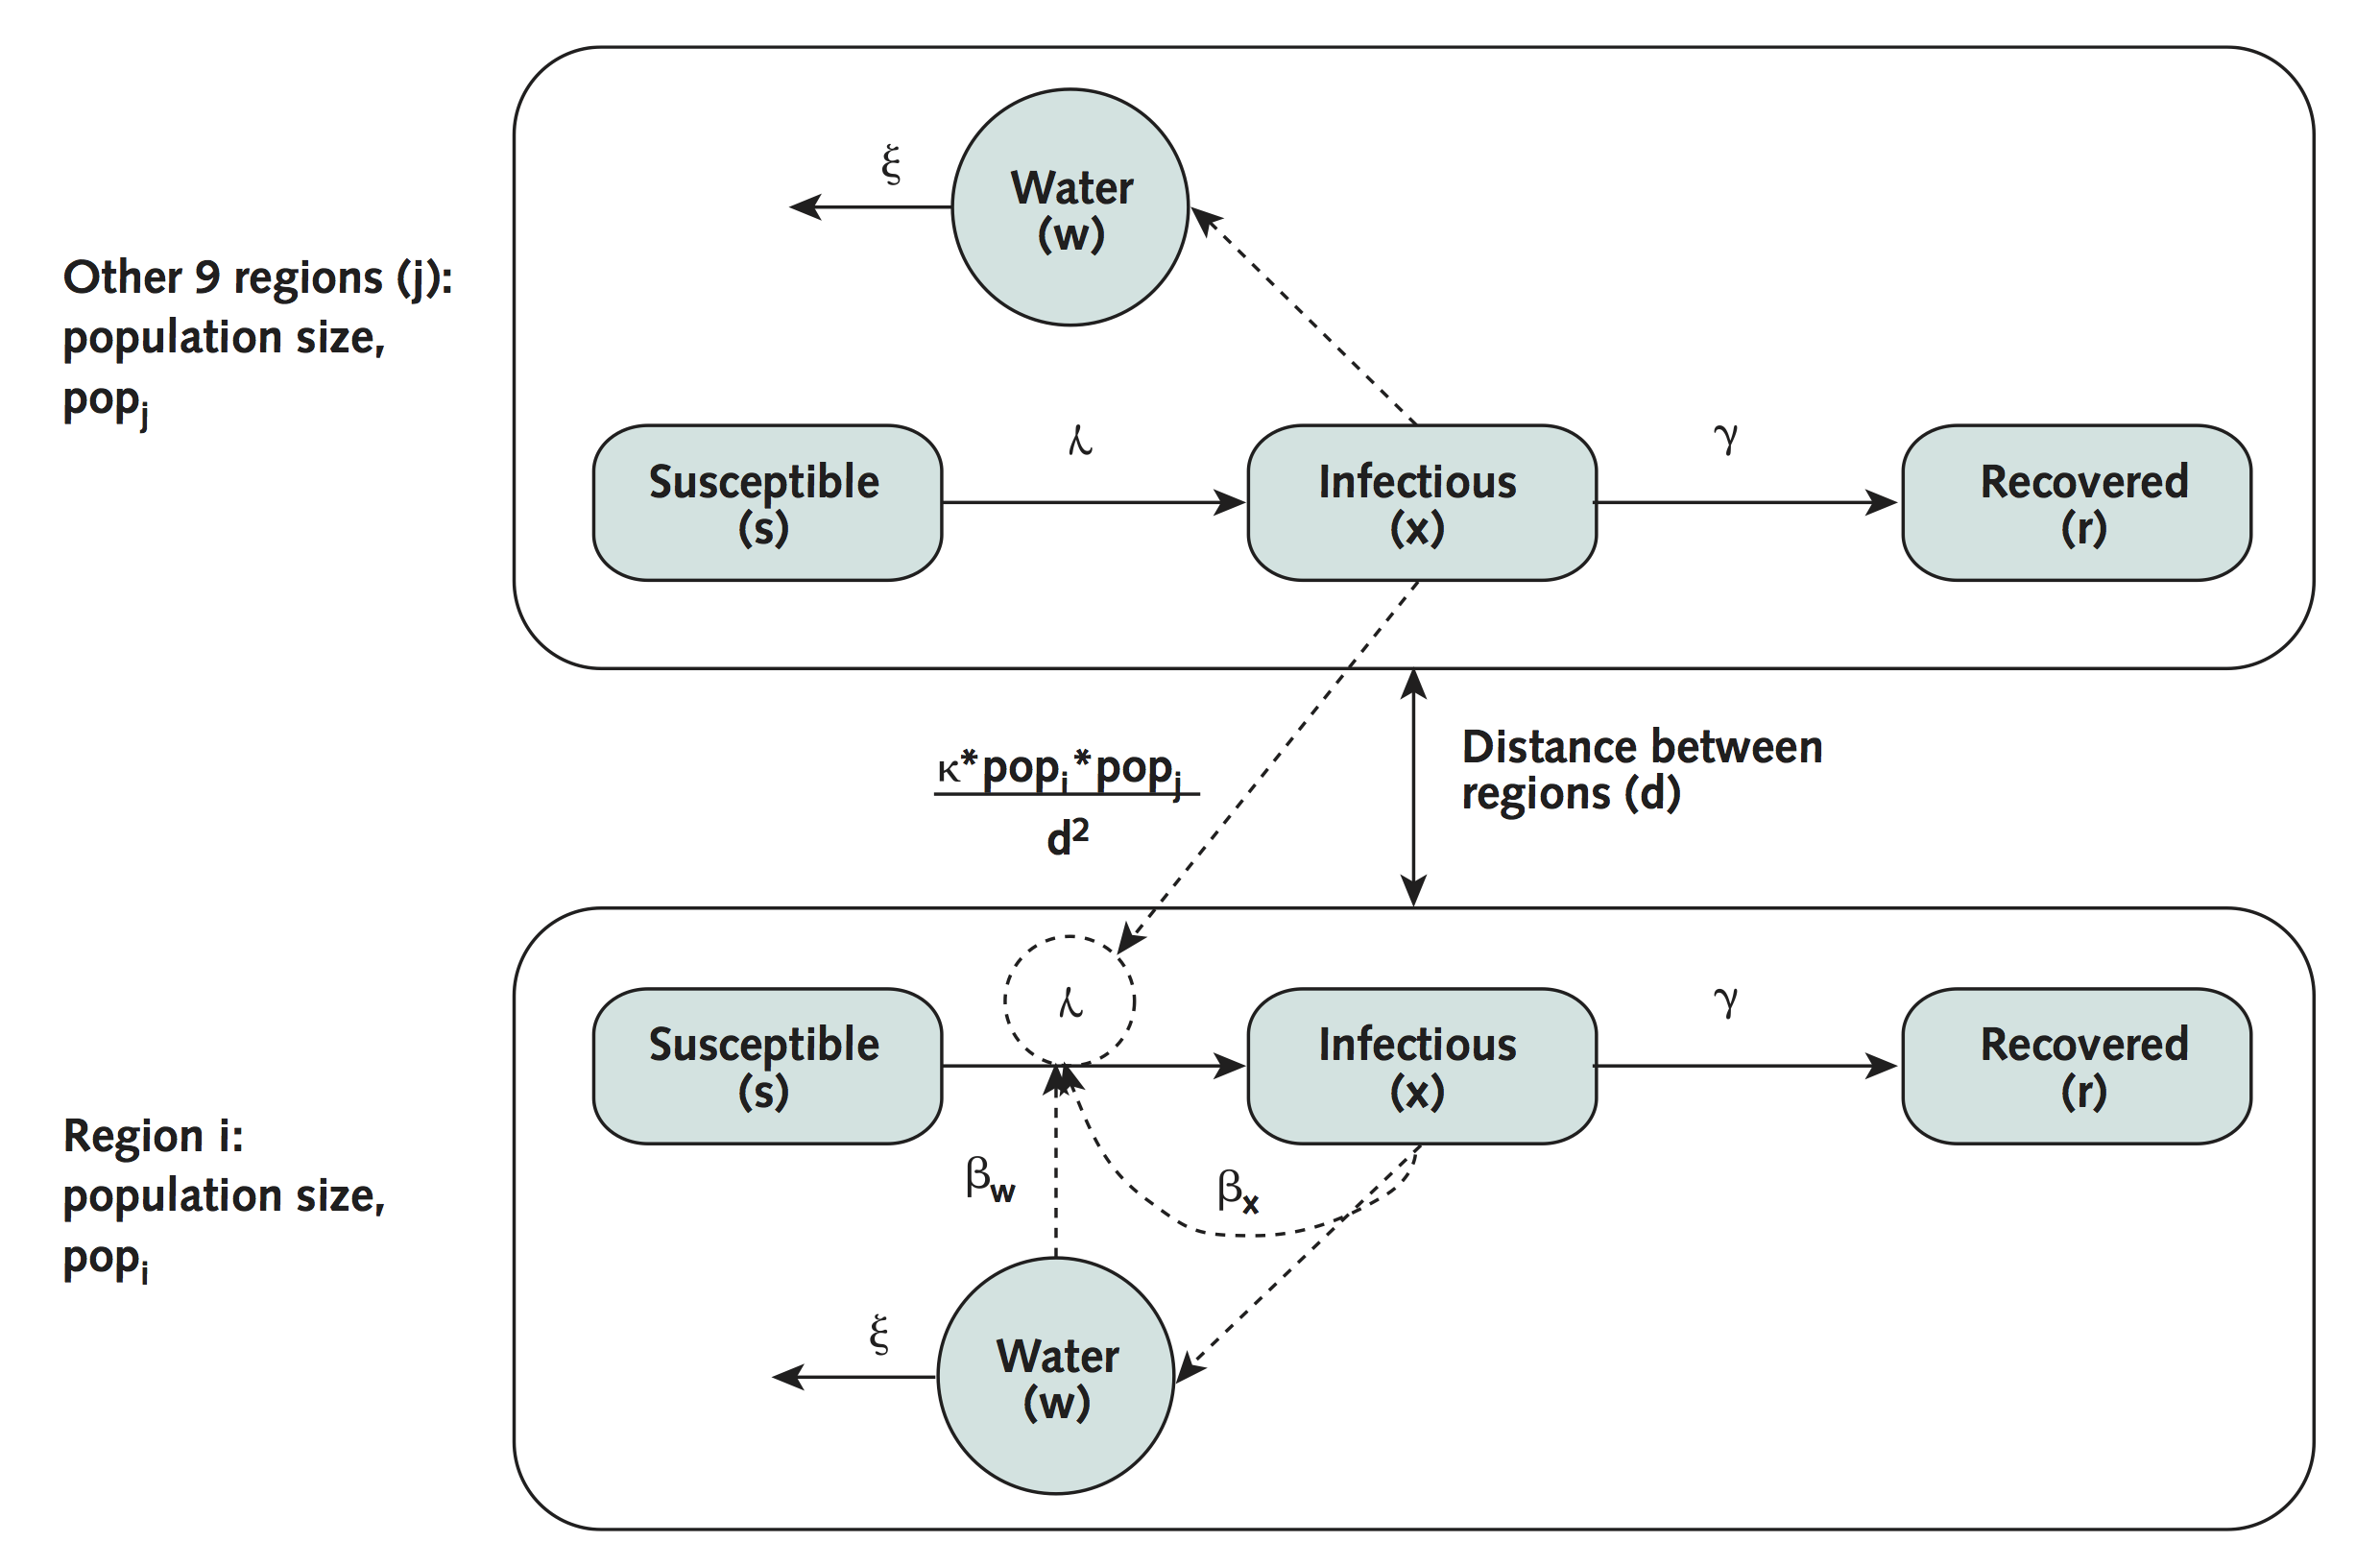
\includegraphics[scale=.9]{Bilder/figure_model_haiti.png}
\caption{Illustration of the SIWR model for several districts. Infectious persons do not only have an effect on their own but also on other districts. Taken from Tuite \textit{et al.} \cite{tuite:2011}.}
\label{pic:model_departments}
\end{figure}
\end{center}


Figure \ref{pic:model_departments} illustrates the processes and compartments and shows which parameter accounts for which process. Each of the ten districts consists of the four compartments susceptible (s), infectious (x), removed (r) and water (w). Birth and natural deaths ($ \mu $) are left out in the figure. $ n $ in the gravity model is set to 2 here. Right calibration of every model is crucial to produce results that are close to reality. As the SIWR model has several parameters, this task is quite difficult. With the onset of disease-control interventions the basic reproductive number $ R_{0} $ is bound to decrease. This process can be taken into account by making $ R_{0} $ time-dependent. This effective reproductive number $ R_{t} $ could look like this with $ f $ a discount factor \cite{tuite:2011}.


\begin{center}
\begin{minipage}[t]{0.6\textwidth}

\begin{equation}
R_{t}=\dfrac{R_{0}}{(1+f)^{t}}
\label{eq:rep_number}
\end{equation}
\end{minipage}
\end{center}
\newline








\newpage
\section{Implementation}
In this section we will describe the implementation of the SIR model in Matlab. To explain why we decided on the SIR and not the SIWR model, we will also look at some of the difficulties of implementing the SIWR model.

\subsection{Problems with rescaling}
We first tried to rescale our model as proposed by Tien and Earn \cite{tien:2010}. It seems, though, that their rescaled model equations are somewhat paradoxical. Looking at the dimensions of equation \eqref{eq:SIWR_susceptible}} there already seems to be some contradiction. The dimension of $\.{s}$,s,i and r is $km^{-2}$. The dimension of $\mu$, $\beta_{w}$ and $\beta_{i}$ is declared as $day^{-1}$ \cite{tien:2010}. This shows that the dimensions on the left and right side of the equation cannot be the same. Because of this, we decided to let our susceptible, infectious and removed compartments have the dimension of percentages. As a consequence, we do not know what dimensions our coefficients have (e.g. $day^{-1}$ or $cells*ml^{-3}$). We will not be able to make the same conclusions as Tuite et al \cite{tuite:2011}. Primarily, we will be able to make qualitative statements about the proportions of transmission caused by the local population versus the interdepartmental transmission.


\subsection{Data from the MSPP}
We collected the raw data from the Minist\`{e}re de la Sant\'{e} Publique et de la Population de la R\'{e}publique d'Haiti (MSPP) \cite{web:MSPP}. To get our ten districts, we added the numbers from Port-au-Prince to the department Ouest. In total, we collected the data for 92 days (the months November and December 2010 and January 2011) and ten different districts. To compare the original data to the model output we needed the amount of susceptible, infectious and removed in each department. Whilst extracting all the data we found some inconsistencies within the data sheets themselves. For this reason we chose to take the data from what we considered the most reliable on the sheets (mainly the data from hospitals). The infectious data were taken directly from the data sheets as the number of hospitalizations. The removed data are the sum of deaths in hospital and the healed. The susceptible data were calculated as the total population minus the infectious and removed. All the values were divided by the respective total population to produce the percentages.\\
One of the bigger problems with the SIWR model is the lack of knowledge about cholera and the water quality during the epidemic. Because we found no data available in the internet and Tuite et al. \cite{tuite:2011} don't cite any source for their data, we started out by setting all the values for the water quality on day 1 to 0. The amount of cholera bacteria would rise due to the bacterial shedding rate from the infected to the water compartment. After some trial runs we discovered that the SIWR model is extremely sensitive to changes in the initial conditions of the water quality. This was one of the main reasons we decided to use the SIR model. Continuing with the SIWR model would result in a high uncertainty about the variability caused by the false initial conditions of the water quality versus the parameters fitted by the solver.






\subsection{Differential equations}
In order to observe intercompartmental transmission, we used the same modification as Tuite et al. \cite{tuite:2011} in their SIWR model. The force of infection $\lambda$ in the \textit{i}th district is:

\begin{center}
\begin{minipage}[t]{0.6\textwidth}

\begin{equation}
\lambda_{i} = \beta_{Xi} x + \sum\limits_{j=1}^I  \Theta_{ij}  x_{j}
\label{eq:lambda}
\end{equation}
\end{minipage}
\end{center}
\newline


The influence of infection of the \textit{jth} district on the \textit{ith} district $\Theta$ is calculated the same way as Tute et al.
Also as stated by Tuite et al., within the short time period that we observe the natural birth/death rate is of no significance \cite{tuite:2011}. This reduces our SIR model equations to:


\begin{center}
\begin{minipage}[t]{0.6\textwidth}

\begin{empheq}[]{flalign}
&\.{s} = - \lambda s&                \label{eq:sir_susceptible} \\
&\.{x} = \lambda s - \gamma x&       \label{eq:sir_infectious} \\
&\.{r} = \gamma x&                   \label{eq:sir_removed}
\end{empheq}
\end{minipage}
\end{center}
\newline



The benefit of this simplified model is that we only need to fit a few coefficients. As a consequence, our fit will most probably be worse than the fit by the SIWR model. 


\subsection{Creation of the solver}
\label{sec:creation of the solver}



Our goal was to build a solver which, starting from our given initial conditions, tries to find the optimal values of the coefficients to reduce the sum of the squared residuals (SSQ). The SSQ is calculated by squaring the difference of the predicted percentage of a compartment (e.g. susceptible, infected or removed) and the observed data and summing them up over all days and districts. Because our model is practically unable to reproduce the observed data for the susceptible compartment we did not include the SSQ of x within the solver criteria. The solver would stop calculating if either the difference of the two following SSQ was smaller than 0.001\% or if the solver has calculated more than 1000 cycles. This was introduced to exclude any infinite loops. In each cycle of the solver, all the coefficients were slightly increased and decreased by 2\% of its value. These modified coefficients were then combined to create all possible scenarios. This results in $2^{k}$ scenarios where k is the number of coefficients that need to be fitted. Because of our simplification to the model we only needed to fit $\kappa$, $\beta_{x}$ and $\gamma$. In each cycle our solver calculated 8 different scenarios. Table \ref{tab:solverbuild} shows the different scenarios calculated.



\begin{table}[htb]
\caption{Table with the 8 scenarios, + representing a 2\% increase and - a 2\% decrease of the coefficient }
\centering
\begin{tabular}{|c|c|c|}
\hline 
$\kappa$ & $\beta_{x}$ & $\gamma$ \\ 
\hline 
+ & + & + \\ 
\hline 
+ & + & - \\ 
\hline 
+ & - & + \\ 
\hline 
+ & - & - \\ 
\hline 
- & + & + \\ 
\hline 
- & + & - \\ 
\hline 
- & - & + \\ 
\hline 
- & - & - \\ 
\hline 
\end{tabular} 
\label{tab:solverbuild}
\end{table}




The solver computes the SSQ starting with these slightly modified coefficients and chooses the ones where the SSQ was reduced the most. The next cycle is then started with these coefficients.\\
We decided to build our own solver mainly for two reasons:

\begin{enumerate}
\item We did not find any adequate solver in the internet for the format of our data
\item We thought it might be an interesting challenge to build one ourselves as a learning experience
\end{enumerate}

Because this is not an established solver there are a few things one has to keep in mind. We tested the consistency of the solver by running the program up to 50 times with the same initial conditions. In each case the result was the same. To test the sensitivity of the solver to different initial conditions we let the whole program run with different starting values of coefficients. This is explained in section \ref{sec:initial conditions}. Another weakness of the solver is that it never lets a parameter stay the same but either increases or decreases its value. This could be excluded by adding a third scenario value, where the parameter does not change. The formula for the total amount of scenarios is $scenarios=n^{k}$ where n is the number of different value changes and k the number of coefficients being fitted. This can result in a large amount of calculations. We decided that the possible inaccuracy of 2\% of the coefficients has a small effect on the overall fit and proceeded with only two value changes in the solver.



\subsection{Initial conditions}
\label{sec:initial conditions}
In our model we not only have initial conditions for the compartments susceptible, infected and removed, but also for the coefficients fitted by the solver. The starting values for the compartments were simply taken from the observed data day 1 (so 1st November 2010). The coefficients of the model were estimated beforehand by simple nonlinear parameter fitting. Based on these calculations we defined an interval of possible values for $\kappa$, $\beta_{x}$ and $\gamma$. Because we decided on a different rescaling method we could not rely on the parameter values given by Tuite et al. \cite{tuite:2011}. Similar to the method used in our solver, we created different scenarios with all the combinations of starting values. This resulted in $4^{3}=64$ different scenarios. To calculate the final model we chose the fitted coefficients from the scenario with the smallest overall SSQ. Figure \ref{pic:sir_flow_our} shows the order of events within our program code.



\begin{center}
\begin{figure}
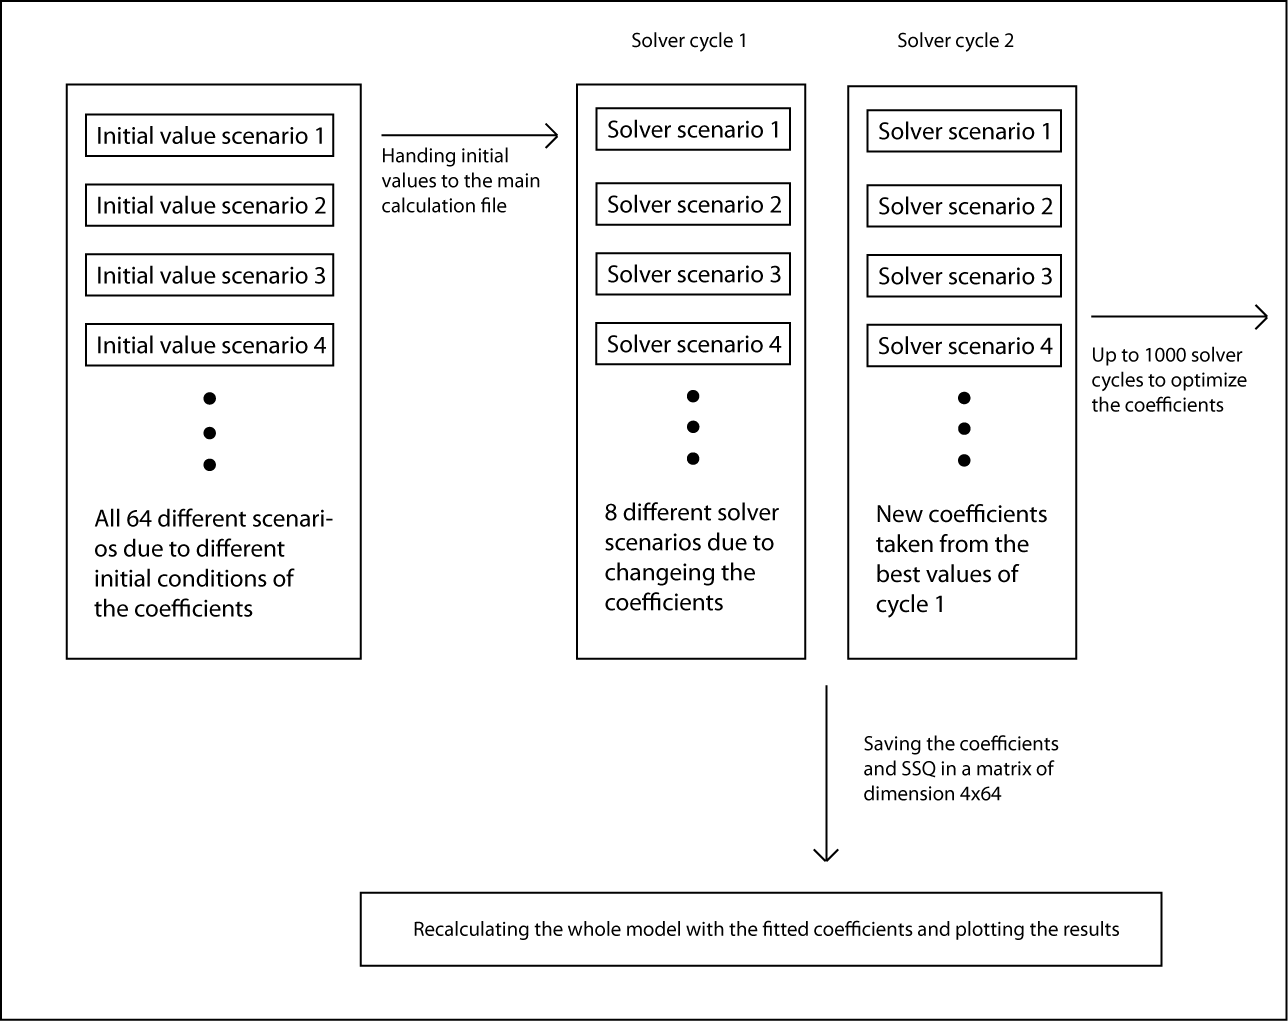
\includegraphics[scale=.6]{Bilder/Matlab_program.png}
\caption{Illustration of the model built by us to clarify the order of events within the code}
\label{pic:sir_flow_our}
\end{figure}
\end{center}




\newpage
\section{Simulation results and discussion}
\subsection{Results of the SIR model}
All the values for the compartments s, x and r calculated by the model are within the possible intervals. The best fit values for $\beta_{x}$, $\gamma$ and $\kappa$ are 3.9114, 3.8816 and 7.5279e-12, respectively. The basic reproductive number $R_{0} = \frac{\lambda S}{\gamma}$ is always smaller than 1 because the product of $\lambda S$ is always smaller than $\gamma$. This would predict a non spreading disease or a very mild epidemic \cite{kermack:1927}. Figures \ref{fig:mean_susceptible} and \ref{fig:mean_removed} show the mean over all districts for the susceptible and removed compartments, respectively. One can see that the slope of the curve is steadier for the calculated model compared to the observed data. The observed curve of the infectious compartment in figure \ref{fig:mean_infectious} is highly nonlinear and the magnitude is slightly earlier than our calculated data. It is important not only to look at the means but the distribution of s, x and r within Haiti.\\

\begin{figure}
  %\centering
  \begin{minipage}[t]{0.49\textwidth}
    \centering
    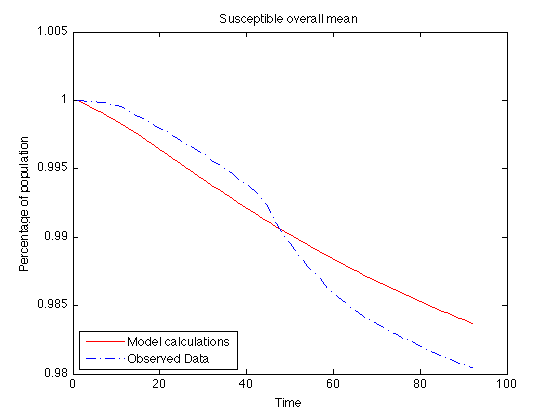
\includegraphics[width=\textwidth]{Bilder/susceptible_mean.png} 
    \caption{Mean over all districts for the susceptible compartment}
	\label{fig:mean_susceptible}
  \end{minipage}
  \hspace{0.02\textwidth}
  \begin{minipage}[t]{0.49\textwidth}
    \centering
    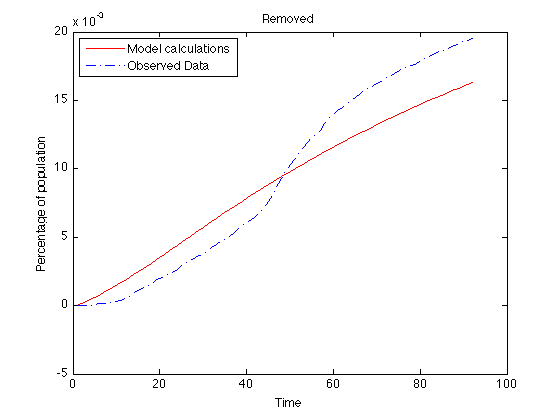
\includegraphics[width=\textwidth]{Bilder/removed_mean.png} 
    \caption{Mean over all districts for the removed compartment}
	\label{fig:mean_removed}
  \end{minipage}
\end{figure}


The plots \ref{fig:all_susceptible}, \ref{fig:all_removed} and \ref{fig:all_infectious} show the observed and calculated values of all ten compartments. The districts Nord, Nord-Est and Grand Anse show an incredible increase and decrease in the removed and susceptible compartments, respectively. These compartments also have unlikely observed data for the infectious compartment, as seen in figure \ref{fig:all_infectious}. In the district Grand Anse the amount of infected people decreases from  0.1\% to 0.04\% within around 3 days. On the other hand, there are some extremely good fits, for instance in the departments Nord-Ouest and Centre. 


\begin{figure}
  %\centering
  \begin{minipage}[t]{0.49\textwidth}
    \centering
    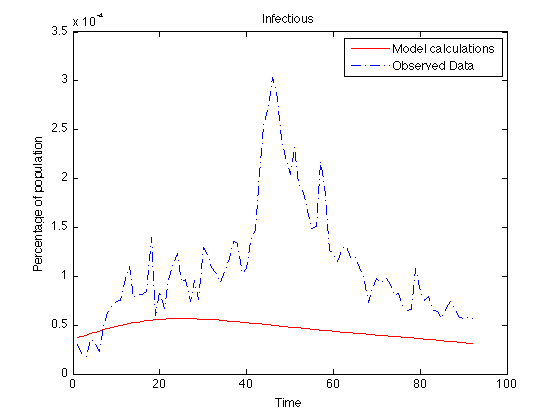
\includegraphics[width=\textwidth]{Bilder/infectious_mean.png} 
    \caption{Mean over all districts for the infectious compartment}
	\label{fig:mean_infectious}
  \end{minipage}
  \hspace{0.02\textwidth}
  \begin{minipage}[t]{0.49\textwidth}
    \centering
    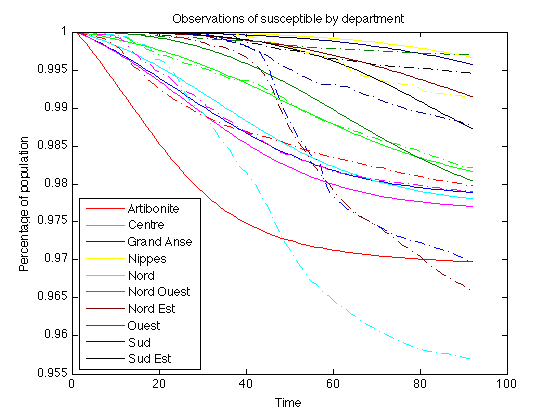
\includegraphics[width=\textwidth]{Bilder/susceptible.png} 
    \caption{Observed and calculated data for all districts of the susceptible compartment}
	\label{fig:all_susceptible}
  \end{minipage}
  
  \hspace{0.15\textwidth}

  %\centering
  \begin{minipage}[t]{0.49\textwidth}
    \centering
    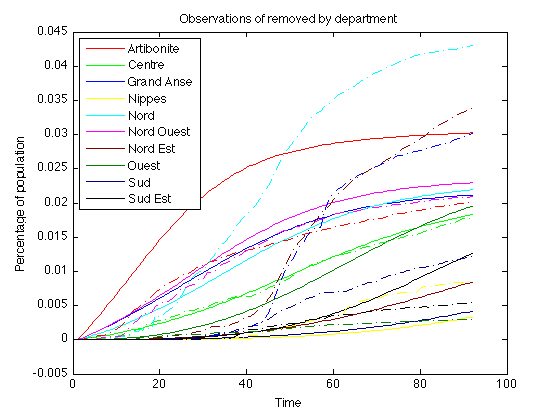
\includegraphics[width=\textwidth]{Bilder/removed.png} 
    \caption{Observed and calculated data for all districts of the removed compartment}
	\label{fig:all_removed}
  \end{minipage}
  \hspace{0.02\textwidth}
  \begin{minipage}[t]{0.49\textwidth}
    \centering
    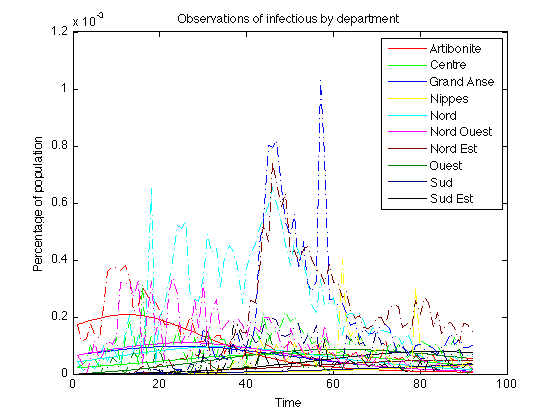
\includegraphics[width=\textwidth]{Bilder/infectious.png} 
    \caption{Observed and calculated data for all districts of the infectious compartment}
	\label{fig:all_infectious}
  \end{minipage}
\end{figure}

One of the benefits of our simple model is the possibility to compare the effect of transmission within the same district versus transmission between districts. The force of infection $\lambda$ consists of two parts, as seen in equation (lambda). Here $\beta_{x}x$ represents the transmission within the same district and $\sum\limits_{j=0}^I  \Theta_{ij}  x_{j$ the transmission between compartments. Figure XX shows the interdepartmental transmission coefficients over time. The best fit of $\beta_{x}=3.9114$ is always around $10^4$ times bigger. This predicts that in our model the transmission within the same district is much more important than the interdepartmental transmission.


\begin{figure}
  %\centering
  \begin{minipage}[t]{\textwidth}
    \centering
    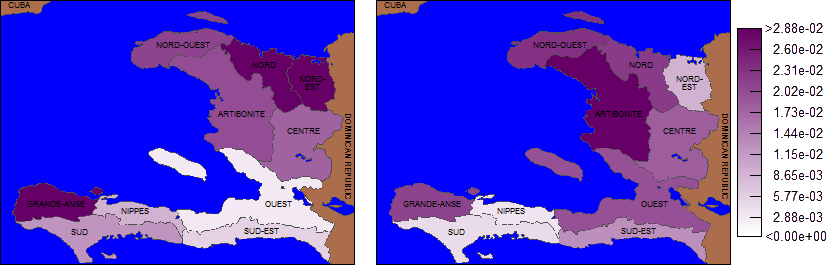
\includegraphics[width=\textwidth]{Bilder/geo_removed.png} 
    \caption{Geographical display of observed and calculated removed data at t=92}
	\label{fig:geo_removed}
  \end{minipage}
\end{figure}

Figure \ref{fig:geo_removed} shows the spread of the removed compartment on the 1st of January 2011. Here the observed data is shown on the left while our calculated data is on the right. Our model predicts the spatial spread of the disease to some extent quite well. After the change of initial conditions in the infectious compartment for the district Grand Anse we were able to also predict the spread in the far west. Our calculated least-infected districts are Sud and Nippes. The observed data show that they are further to the east, namely Ouest and Sud-Est. Our model also calculates the highest-infected district to be Artibonite, whereas the observed data shows that they are Nord-Est and Nord.



\subsection{Discussion} 
The reliability and accessibility of data have proved to be a crucial part of building this model. Because of the lack of water quality data we have decided to construct an ordinary SIR model instead of an SIWR. Even with our simplified SIR model equations we were able to predict the epidemic over 3 months to some extent. In our model, the interdepartmental transmission is of no importance to the spread of the disease. There are two main reasons we believe why this might be in our model. Tien and Earn \cite{tien:2010} put the percentage of infected, susceptible and infectious populations in relation to the area observed in the model. For us this would mean we put the respective percentages in relation to the area of the districts. The result would be a density, for instance percent infected per square kilometer. For districts with many inhabitants in a relatively small area this would result in much higher values for s,x and r compared to sparsely inhabited districts. When using the gravity model as proposed by Tuite et al. \cite{tuite:2011} the districts with a high x would have a much greater influence on the force of infection $\lambda$.\\
Another reason might be the gravity model we used in itself. Because we chose a different way of rescaling our values, s,x and r are much higher than those calculated by Tuite et al. \cite{tuite:2011}. As a result the relation $\frac{pop_{i}*pop_{j}}{d^{n}}$ might be unsuited for our dimensions. We tried to even this out by fitting $\kappa$. Even so our $\kappa$ of 7.5279e-12 is hardly bigger than the one calculated by Tuite et al. of 6.83e–12 \cite{tuite:2011}. Looking at the observed data we tried to find a reason for the sudden spread of the disease in the Grand Anse, Nord Est and Nord districts. In the aftermath of the earthquake, around 400,000 Haitians were evacuated to Jeremie, the capital city of Grand Anse \cite{web:appo}. The density of refugees and fast deplention of ressources within Grand Anse could be a possible factor for the quick propagation of cholera within the local population. For future modeling of disaster related epidemics we propose to not only try a gravity weighted model to predict interdepartmental transmission, but also to look at possibilities to model the mobility of the population between districts, the exact flow of waterways to predict possible futher contamination of surface water reservoirs and to include the shift of population in the aftermath of the disaster for possible effects on the transmission of the pathogen.









\newpage
\section{Summary and Outlook}
\subsection{Summary}
We tried to model the 2010/2011 cholera epidemic with the SIWR model proposed by Tien et al. \cite{tien:2010} and adjusted by Tuite et al. \cite{tuite:2011}. After having trouble to reproduce the model due to possible inconsistencies within the model equations and the lack of reliable data for the water quality, we decided to rescale our model in a different way and to onyl fit an SIR model first proposed by Kermack et al. \cite{kermack:1927} to the data. Using a self built solver to predict the coefficients $\beta_{x}$, $\kappa$ and $\gamma$ we were able to reproduce the spacial distribution and magnitude of the two compartments S and R. 
Further improvements to the model were proposed to increase the possibility to model an epidemic such as the 2010 cholera outbreak with SIR/SIWR models.


\subsection{Outlook}
In response to the cholera outbreak, the Haitian government and partner agencies initiated emergency public health response activities aimed at treating suspected cholera cases and preventing new ones. Response activities included mass media cholera campaigns through the radio, hygiene promotion activities by community health workers, distribution of water purification tablets and soap, and limited distribution of oral rehydration solution (ORS) sachets \cite{web:ors}. Regarding the mass media campaign, it would be more effective if we understood the distribution of the cholera bacteria in waterways. With our model it is unfortunately not yet possible to do so. Our model needs more detailed information, which is currently not available. In the case of a future epidemic it would be important not only to gather data about the infected and recovered populations, but also to collect information on water quality, i.e. cholera bacteria concentrations, and the consumption of drinking water from surface water reservoirs.\\
We believe such a dataset would greatly improve the possibility of modelling a system such as a cholera epidemic, like the one in Haiti in 2010.
\newpage

\listoffigures

\listoftables
\newpage




\section{References}
\bibliographystyle{plain}
\bibliography{Citations/cholera.bib}




\end{document}  
